\section{Neutron Sources}

\subsection{High-Flux Neutron Reactors}

There are 250 or so research reactors in 55 countries \cite{researchreactorstats}, and a number of these are used for materials research.  In the UK, there is only one remaining research reactor, and this is the Neptune pool type reactor at Rolls Royce\cite{neptunereactor}.  In Cadrache, France, the Jules Horowitz reactor is under construction and this is being built specifically as a materials testing reactor.  It will be crucial in researching new materials for use in upcomming Gen IV nuclear power stations \cite{researchreactorstats}.  


\subsubsection{High Flux Isotope Reactor, Oak Ridge}

The High Flux Isotope Reactor, at the Oak Ridge National Laboratory in America, is an 85MW research reactor that provides testing space within the reactor as well as a number of neutron beam lines.  The reactor uses highly enriched Uranium as its fuel source and is scheduled to operate at 100% capacity for 161 days per year, in cycles of approximately 23 days.  A 30cm surround of Beryllium is used to reflect neutrons, and in the reactor core there is a high flux of thermal neutrons at a rate of $2.3 x 10^15$ neutrons $cm^{-2} s^{-1}$\cite{hfirornluserguide}.



\begin{figure}[tbp]
  \begin{center}
    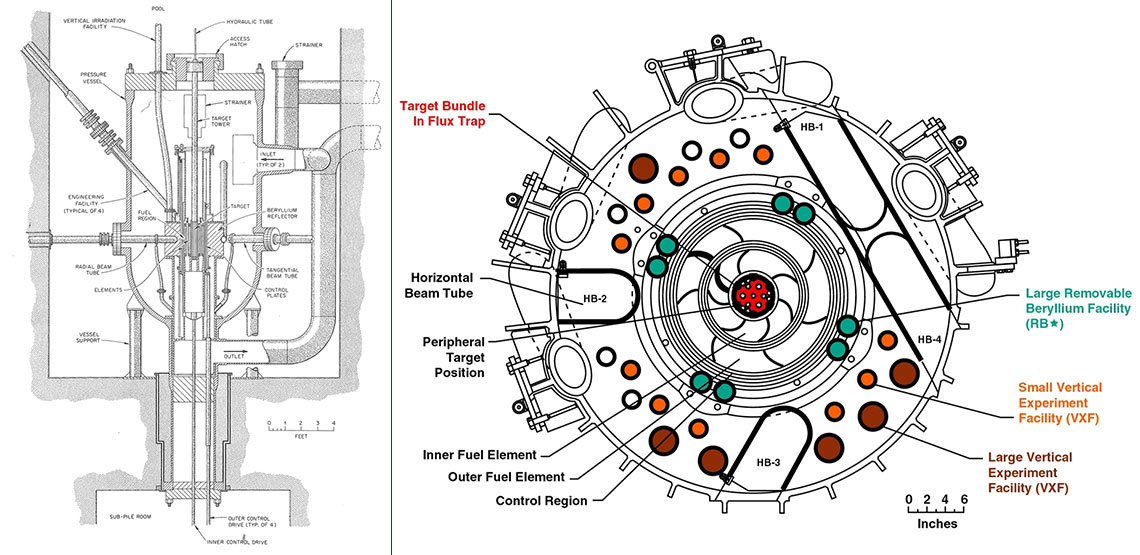
\includegraphics[width=15.0cm]{chapters/background_activity/images/hfir-cross-sections.jpg}
    \captionsetup{font={it}}
    \caption{A cross section of the HFIR \cite{hfirornl}}
    \label{fig:hrirornlfig}
  \end{center}
\end{figure}


\subsubsection{NIST Center for Neutron Research}

The NBS (National Bureau of Standards) Reactor was designed as a research reactor with a power output of 40MW and a neutron flux of approximately $1.0x10^15$ neutrons $cm^{-2} s^{-1}$.  In 2006 it was decided to extend the facility and add beam lines







\subsection{Spallation}

Neutrons cause fission in nuclear reactors, but spallation sources require protons and high mass targets.  The energy of the protons required is a magnitude greater than that of the Scanditronix MC-40 Cyclotron at the University of Birmingham, with spallation source accelerators having a range from 500MeV to over 1GeV.  



\subsubsection{ISIS}

Ions are attracted from a plasma source and a passed through to a radio frequency quadrupole (RFQ) accerlerator.  The RFQ supplies 665 KeV protons in batches to the linac every 4.94 ns.



